\problemname{Egocentric Expedition}

\illustration{0.4}{flat-earth}{
    Map of the square and stationary earth.
    Public Domain by Prof. Orlando Ferguson on \href{https://commons.wikimedia.org/wiki/File:Orlando-Ferguson-flat-earth-map_edit.jpg}{Wikimedia~Commons}
}%

\newcommand{\maxt}{10^4}
\newcommand{\maxx}{50}
\newcommand{\maxd}{50}

%\problemQuote{Whenever things were frightening, it was a good idea to measure them.}{Daniel Kehlmann}

You are the famous explorer \emph{Christopherus Columb} and unlike most of your contemporaries you know that the earth and the world is flat and a perfect square.
While others dreamfully deluded themselves with the fanatic heliocentric gospel that the earth orbits the sun, you in your superior wisdom discerned the higher truth of egocentrism: you alone remain, naturally, at the center of the world.

The only lifetime achievement remaining, worthy of your name, is to determine the exact area of the world.
You cannot sail to the edge of the world yourself, as the world moves along with you such that you continue to be the center of the world.
Therefore, you have to send your subordinates.
They sail in a straight line direction chosen by you, starting at the center of the world.
After their return, they will report the distance from you to the edge of the world in that direction.

As most crew members have been lured away by the heretic masses, there are only enough crew members left to operate a single ship.
Knowing that there is barely enough time to send this ship out \emph{twice}, are you wise enough to determine the area of the world?

\begin{figure}[h]
	\centering
	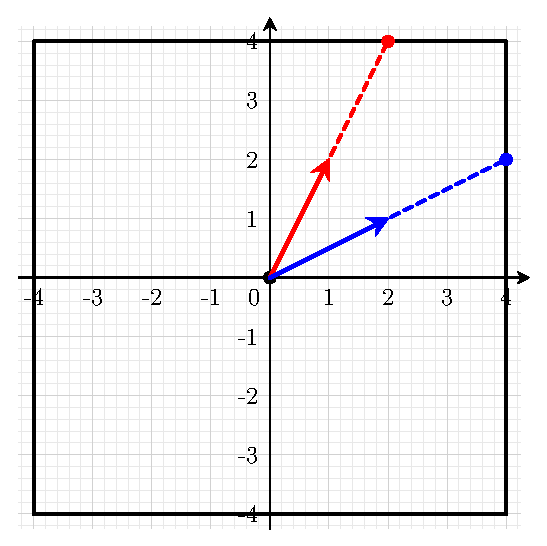
\includegraphics[width=0.3\textwidth]{test1}
	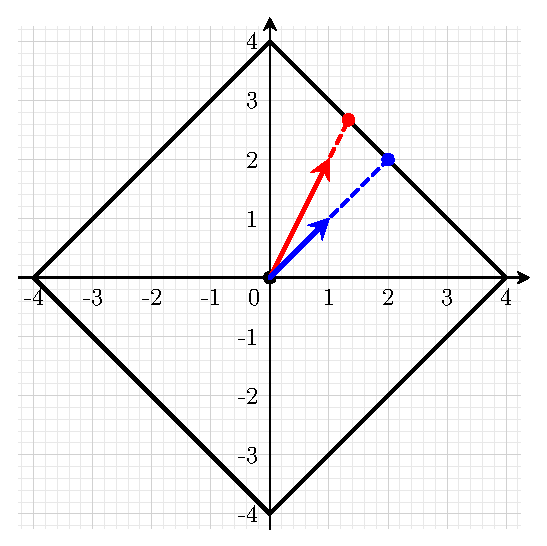
\includegraphics[width=0.3\textwidth]{test2}
	\caption{Visualization of the two test cases used for the sample interaction.
    In the second sample (right), the ship is first sent in \textcolor{red}{direction $(1, 2)$}, where it finds the edge of the world at $\approx (1.33, 2.67)$, reporting distance $\approx 2.98$.
    Then the ship is sent again in \textcolor{blue}{direction $(1, 1)$}, finding the edge at $(2, 2)$, reporting distance $\approx 2.83$.}
\end{figure}

Note that the rotation of the world square can be arbitrary, and the corner coordinates of the world do not have to be integer.

\begin{Interaction}
	This is an interactive problem.
    Your submission will be run against an \emph{interactor},
    which reads from the standard output of your submission
    and writes to the standard input of your submission.
    This interaction needs to follow a specific protocol:

	The interactor first sends one line with an integer $t$ ($1 \leq t \leq \maxt$), the number of test cases.

    For each test case, you can ask \emph{at most two} queries.

    For every query, output ``\texttt{?~$x$~$y$}'' ($0 \leq \left| x \right|$,~$\left| y \right| \leq \maxx, (x, y) \neq (0, 0)$), where $x$ and $y$ are integers, and $(x, y)$ is the direction you send a ship to.

	The interactor will respond to each query with one line containing a real value $d$ ($0 < d \leq \maxd$), the distance the ship reported.
    This distance $d$ is given with exactly $10$ decimal places, and has an absolute \emph{and} relative error of at most $10^{-7}$.

    After up to two queries, you should output ``\texttt{!~A}'', where $A$ is an integer, the area of the square.
	It is guaranteed that the square always has a positive integer area.

	The interactor is not adaptive: the borders of the world are fixed before the first query.

    Make sure you \textbf{flush} the standard output after every output.
    For example, you can use \texttt{fflush(stdout)} in C++, \texttt{System.out.flush()} in Java, \texttt{sys.stdout.flush()} in Python, \texttt{std::io::stdout().flush()} in Rust, and \texttt{hFlush stdout} in Haskell.

    A \emph{testing tool} is provided to help you develop your solution.
\end{Interaction}
